\documentclass[12pt, leqno]{article} %% use to set typesize
\input{common}

\begin{document}
\hdr{2019-05-22}

\section{Optimality conditions}

In an unconstrained problem with a differentiable objective
function, a necessary (but not sufficient) condition for $x_*$
to be a local minimizer is that $\phi'(x_*) = 0$.
For intuition, picture a function $\phi : \bbR^n \rightarrow \bbR$; if
you'd like to be concrete, let $n = 2$.  Absent a computer, we might
optimize $\phi$ by the physical experiment of dropping a tiny ball
onto the surface and watching it roll downhill (in the steepest
descent direction) until it reaches the minimum.  The statement
that $\phi'(x_*) = 0$ (or that $\nabla \phi(x_*) = 0$) basically means
the function looks flat at $x_*$ to a sufficiently near-sighted observer;
if $\phi'(x_*)$ is not zero, then $x_* - \epsilon \nabla \phi(x_*)$
will be a little bit ``downhill'' of $x_*$; that is,
if $\|\nabla \phi(x_*)\| \neq 0$ then
\[
  \phi(x_* - \epsilon \nabla \phi(x_*)) =
  \phi(x_*) - \epsilon \|\nabla \phi(x_*)\|^2 + o(\epsilon) < \phi(x_*)
\]
for sufficiently small $\epsilon$.

Most students learn the first-order optimality conditions for unconstrained
optimization in a first course, but sometimes that course gets
everyone too stuck on the idea of computing a gradient.  What is
really happening is that the function should be ``flat in all directions,''
i.e.~all directional derivatives are zero.  This is equivalent to the
statement that the gradient is zero, of course, but sometimes it is
notationally easier to check that an arbitrary directional derivative
is zero than to try to write down the gradient.  For example, consider
the quadratic objective
\[
  \phi(x) = \frac{1}{2} x^T A x + x^T b + c.
\]
Now, we will write an arbitrary directional derivative of $\phi$ in
terms of ``variational notation'' (described in the background notes):
\[
\delta \phi(x) =
\left. \frac{d}{d\epsilon} \right|_{\epsilon = 0} \phi(x+ \epsilon \delta x)
= (\delta x)^T (Ax + b).
\]
At a critical point, $\delta \phi(x)$ should be zero for any
choice of $\delta x$, so the stationary point occurs at $Ax_* + b = 0$.
There is a unique minimizer $x_*$ if $A$ is positive definite.
When the number of variables is not too large --- up to a few
thousand, say --- we might solve this system of linear equations
directly using a variant of Gaussian elimination
if we wanted to find the minimizer.  When the number of variables
is much larger, we may prefer to use an iterative method 
to solve the system, e.g.~the method of conjugate gradients (CG).
This method can be interpreted either as an iterative solver for
linear equations or as an iterative optimization method.

Now let's turn to the {\em constrained} case.  Rather than repeating
the formal derivation of the first-order constrained optimality
conditions that you have likely seen before, let me again give you an
interpretation that involves some physical intuition.  For the
unconstrained case, we thought about solving the problem by rolling
a tiny ball down hill until it came to rest.  If we wanted to solve a
constrained minimization problem, we could build a great wall between
the feasible and the infeasible region.  A ball rolling into the wall
would still roll freely in directions tangent to the wall (or away
from the wall) if those directions were downhill; at a constrained
miminizer, the force pulling the ball downhill would be perfectly
balanced against an opposing force pushing into the feasible region
in the direction of the normal to the wall.  If the feasible region
is $\{x : c(x) \leq 0\}$, the normal direction pointing inward at a
boundary point $x_*$ s.t.~$c(x_*) = 0$ is proportional to
$-\nabla c(x_*)$.  Hence, if $x_*$ is a constrained minimum,
we expect the sum of the ``rolling downhill'' force ($-\nabla \phi$)
and something proportional to $-\nabla c(x_*)$ to be zero:
\[
  -\nabla \phi(x_*) - \mu \nabla c(x_*) = 0.
\]
The {\em Lagrange multiplier} $\mu$ in this picture represents the
magnitude of the restoring force from the wall balancing the tendency
to roll downhill.

More abstractly, and more generally, suppose that we have a mix of
equality and inequality constraints.  We define
the {\em augmented Lagrangian}
\[
  L(x, \lambda, \mu) = \phi(x) +
    \sum_{i \in \mathcal{E}} \lambda_i c_i(x) +
    \sum_{i \in \mathcal{I}} \mu_i c_i(x).
\]
The {\em Karush-Kuhn-Tucker (KKT) conditions} for $x_*$ to be a
constrained minimizer are
\begin{align*}
  \nabla_x L(x_*) &= 0 \\
  c_i(x_*) &= 0, \quad i \in \mathcal{E}
  & \mbox{equality constraints}\\
  c_i(x_*) & \leq 0, \quad i \in \mathcal{I}
  & \mbox{inequality constraints}\\
  \mu_i & \geq 0, \quad i \in \mathcal{I}
  & \mbox{non-negativity of multipliers}\\
  c_i(x_*) \mu_i &= 0, \quad i \in \mathcal{I}
  & \mbox{complementary slackness}
\end{align*}
where the (negative of) the ``total force'' at $x_*$ is
\[
  \nabla_x L(x_*) = \nabla \phi(x_*) +
    \sum_{i\in \mathcal{E}} \lambda_i \nabla c_i(x_*) +
    \sum_{i\in \mathcal{I}} \mu_i \nabla c_i(x_*).
\]
The complementary slackness condition corresponds to the idea that a
multiplier should be nonzero only if the corresponding constraint is
active (a ``restoring force'' is only present if our test ball
is pushed into a wall).

Like the critical point equation in the unconstrained case, the KKT
conditions define a set of (necessary but not sufficient) nonlinear
algebraic equations that must be satisfied at a minimizer.  I like to
think about the ``rolling downhill'' intuition for these necessary
conditions because it suggests a way of thinking about numerical
methods.

For completeness, we will say a few brief words about
the second-order {\em sufficient} conditions for optimality.
In the unconstrained case, $x_*$ is a strong
local minimizer of $\phi$ if $\nabla \phi(x_*) = 0$ and
the Hessian matrix $H_{\phi}$ is positive definite; that is because
in this case $x_*$ is the strong minimizer of the quadratic approximation
\[
  \phi(x) \approx \phi(x_*) + \frac{1}{2} (x-x_*)^T H_\phi(x_*) (x-x_*).
\]
In the constrained case, the Hessian only needs to be positive
definite for those $u$ that are orthogonal to $\nabla c_i(x_*)$
for each $c_i$ that is active (has a nonzero Lagrange multiplier).
We will see this idea in two weeks when we talk about kernel methods,
and in particular talk about the idea of
a {\em conditionally positive definite} kernel function.

%% \section{Numerical methods}

%% With our lightning review of some fundamental theory out of the way,
%% it is time to turn to numerical methods!  After discussing least
%% squares (which we can solve by direct methods), we will spend
%% the next three lectures talking about gradient and stochastic gradient
%% methods, Newton and Gauss-Newton, and (block) coordinate descent.
%% We will see additional solver ideas as we move through the semester,
%% but these are nicely prototypical examples that illustrate two running
%% themes in the design of numerical methods for optimization.

%% \paragraph{Fixed point iterations}
%% All our nonlinear solvers (and some of our linear solvers) will be
%% {\em iterative}.  We can write most as {\em fixed point iterations}
%% \begin{equation}
%%   x^{k+1} = G(x^k), \label{eq:fixed-point}
%% \end{equation}
%% which we hope will converge to a fixed point, i.e. $x^* = G(x^*)$.
%% We often approach convergence analysis through the
%% {\em error iteration} relating the error $e^k = x^k-x^*$ at
%% successive steps:
%% \begin{equation}
%%   e^{k+1} = G(x^* + e^k)-G(x^*).
%% \end{equation}

%% As a teaser for this sort of analysis, consider one of the simplest
%% algorithms I know: gradient descent with a fixed step size $h$, applied
%% to the quadratic model problem
%% \[
%%   \phi(x) = \frac{1}{2} x^T A x + b^T x + c
%% \]
%% where $A$ is assumed to be symmetric and positive definite.  The
%% algorithm produces iterates
%% \begin{align*}
%%   x^{k+1}
%%   &= x^k - h \nabla \phi(x^k) \\
%%   &= x^k - h (Ax^k + b) \\
%%   &= (I-hA) x^k - h b.
%% \end{align*}
%% Now we subtract the fixed point equation for the true solution $x^*$
%% in order to get an error iteration:
%% \begin{align*}
%%     & [x^{k+1} = (I-hA) x^k - hb] \\
%%   - & [x^*     = (I-hA) x^* - hb] \\ \hline
%%   = & [e^{k+1} = (I-hA) e^k ]
%% \end{align*}
%% where $e^k = x^k-x^*$.  The error iteration converges iff the largest
%% eigenvalue of $A$ is less than $2 h^{-1}$; if this condition is
%% satisfied, then
%% \[
%%   \|e^{k+1}\| \leq (1-h\lambda_{\max}(A)) \|e^k\|
%% \]
%% and so we have $\|e^{k+1}\| \leq (1-h\lambda_{\max}(A))^{k+1} \|e^0\|$,
%% a convergence rate which is known as (R)-linear convergence or
%% as geometric convergence, depending on which corner of the literature
%% one prefers to read.

%% \paragraph{Model-based methods}
%% Most nonquadratic problems are too hard to solve directly.  On the other
%% hand, we can {\em model} hard nonquadratic problems by simpler (possibly
%% linear) problems as a way of building iterative solvers.  The most
%% common tactic --- but not the only one! --- is to approximate the
%% nonlinear function by a linear or quadratic function and apply all the
%% things we know about linear algebra.  We will return to this idea in
%% the next lecture when we discuss Newton-type methods for optimization.


\section{Cricket chirps: an example}

Did you know that you can estimate the temperature by listening to the
rate of chirps?  The data set in Table~\ref{table1}%
\footnote{Data set originally attributed to
  \url{http://mste.illinois.edu}}.  represents measurements of the
number of chirps (over 15 seconds) of a striped ground cricket at
different temperatures measured in degrees Farenheit.  A plot
(Figure~\ref{fig2}) shows that the two are roughly correlated: the
higher the temperature, the faster the crickets chirp.  We can
quantify this by attempting to fit a linear model
\[
  \mbox{temperature} = \alpha \cdot \mbox{chirps} + \beta + \epsilon
\]
where $\epsilon$ is an error term.  To solve this problem by standard linear
regression, we minimize the least squares norm residual
\[
  r = b-Ax
\]
where
\begin{align*}
  b_{i} &= \mbox{temperature in experiment } i \\
  A_{i1} &= \mbox{chirps in experiment } i \\
  A_{i2} &= 1 \\
  x &= \begin{bmatrix} \alpha \\ \beta \end{bmatrix}
\end{align*}
Assuming the measurement error $\epsilon$ is Gaussian, the least
squares procedure gives the {\em maximum likelihood estimate}
estimate for $\alpha$ and $\beta$.

MATLAB and Octave are capable of solving least squares problems using
the backslash operator; that is, if {\tt chirps} and {\tt temp} are
column vectors in MATLAB, we can solve this regression problem as
\begin{lstlisting}
  A = [chirps, ones(ndata,1)];
  x = A\temp;
\end{lstlisting}

\begin{figure}
  \begin{center}
    \begin{tikzpicture}
      \begin{axis}[xlabel={Chirps},ylabel={Degrees},grid=major]
        \addplot[only marks] table {data/cricket.dat};
        \addplot table[x=chirp,y=fit]{data/cricket.dat};
      \end{axis}
    \end{tikzpicture}
  \end{center}
  \caption{Cricket chirps vs.~temperature and a model fit via
    linear regression.}
  \label{fig2}
\end{figure}

\begin{table}
  \small
  \begin{tabular}{l|cccccccccccccccccc}
    Chirp &
    20& 16& 20& 18& 17& 16& 15& 17& 15& 16& 15& 17& 16& 17& 14 \\
    Temp &
    89& 72& 93& 84& 81& 75& 70& 82& 69& 83& 80& 83& 81& 84& 76
  \end{tabular}
  \caption{Cricket data: Chirp count over a 15 second period vs.~temperature
    in degrees Farenheit.}
  \label{table1}
\end{table}

In more complex examples, we want to fit a model involving more than
two variables.  This still leads to a linear least squares problem,
but one in which $A$ may have more than one or two columns.
We also use linear least squares
problems as a building block for more complex fitting procedures,
including fitting nonlinear models and models with more complicated
objective functions.

\section{Normal equations}

\begin{figure}
  \begin{center}
  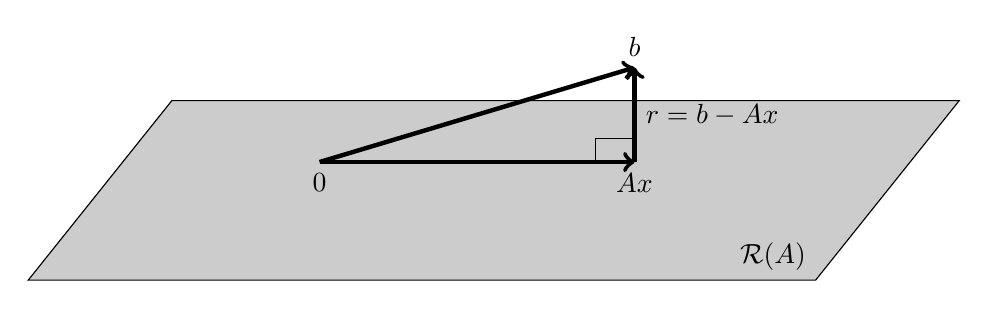
\begin{tikzpicture}
    \begin{scope}[xslant=0.8,xscale=5,yscale=3]
      \draw[fill=black!20] (-0.5,-0.5) rectangle (1.5,0.26);
      \draw[ultra thick,->]
        (0,0) node[below] {$0$} --
        (0.8,0) node[below] {$Ax$};
      \node[above left] at (1.5,-0.5) {$\mathcal{R}(A)$};
    \end{scope}
    \begin{scope}[xscale=5,yscale=3]
    \draw[ultra thick,->]
      (0,0) -- (0.8,0.4) node[above] {$b$};
    \draw[ultra thick,->]
      (0.8,0) -- (0.8,0.4) node[midway,right] {$r=b-Ax$};
    \draw (0.7,0) -- (0.7,0.1) -- (0.8,0.1);
    \end{scope}
  \end{tikzpicture}
  \end{center}
  \caption{Picture of a linear least squares problem.  The vector $Ax$
           is the closest vector in $\mathcal{R}(A)$ to a target
           vector $b$ in the Euclidean norm.  Consequently, the
           residual $r = b-Ax$ is normal (orthogonal) to
           $\mathcal{R}(A)$.}
  \label{fig1}
\end{figure}

The linear least squares problem is a quadratic optimization problem,
and we have already seen that we can write down the solution to such
problems in terms of linear systems of equations.
When we minimize the Euclidean norm of $r = b-Ax$, we find that $r$ is
{\em normal} to everything in the range space of $A$ (Figure~\ref{fig1}):
\[
  b-Ax \perp \mathcal{R}(A),
\]
or, equivalently, for all $z \in \bbR^n$ we have
\[
  0 = (Az)^T (b-Ax) = z^T(A^T b - A^T A x).
\]
The statement that the residual is orthogonal to everything in
$\mathcal{R}(A)$ thus leads to the {\em normal equations}
\[
  A^T A x = A^T b.
\]
To see why this is the right system, suppose $x$ satisfies the normal
equations and let $y \in \bbR^{n}$ be arbitrary.  Using the fact that
$r \perp Ay$ and the Pythagorean theorem, we have
\[
  \|b-A(x+y)\|^2 = \|r-Ay\|^2 = \|r\|^2 + \|Ay\|^2 > 0.
\]
The inequality is strict if $Ay \neq 0$; and if the columns of
$A$ are linearly independent, $Ay = 0$ is equivalent to $y = 0$.

We can also reach the normal equations by calculus.  Define
the least squares objective function:
\[
  F(x) = \|Ax-b\|^2 = (Ax-b)^T (Ax-b) = x^T A^TA x - 2x^T A^T b + b^T b.
\]
The minimum occurs at a {\em stationary point}; that is,
for any perturbation $\delta x$ to $x$ we have
\[
  \delta F = 2 \delta x^T (A^T A x - A^T b) = 0;
\]
equivalently, $\nabla F(x) = 2 (A^T A x - A^T b) = 0$ ---
the normal equations again!

\section{A family of factorizations}

If $A$ is full rank, then $A^T A$ is symmetric and positive definite
matrix, and the normal equations have a unique solution
\[
  x = A^{\dagger} b \mbox{ where } A^{\dagger} = (A^T A)^{-1} A^T.
\]
The matrix $A^\dagger \in \bbR^{n \times m}$ is the
{\em Moore-Penrose pseudoinverse}.
If $m = n$, the pseudoinverse and the inverse are
the same.  For $m > n$, the Moore-Penrose pseudoinverse
has the property that
\[
  A^\dagger A = I;
\]
and
\[
  \Pi = A A^\dagger = Q_1 Q_1^T = U_1 U_1^T
\]
is the {\em orthogonal projector} that maps each vector to the
closest vector (in the Euclidean norm) in the range space of $A$.

Even for small least squares problems, we do not work with the Moore-Penrose
pseudoinverse directly, just as we do not compute explicit inverses of
square matrices.  Instead, we use different {\em matrix factorizations}
to solve the problem.  For least squares problems, the three main
factorizations are Cholesky, QR, and SVD.  Each of these methods costs
$O(n^2 m)$ time to set up a factorization to apply the pseudoinverse,
then $O(nm)$ time per right hand side to actually complete the solve
for a given right hand side.

\subsection{Cholesky}

If $A$ is full rank, then $A^T A$ is symmetric and positive definite
matrix, and we can compute a Cholesky factorization of $A^T A$:
\[
  A^T A = R^T R,
\]
where $R$ is an upper triangular matrix.
The solution to the least squares problem is then
\[
  x = (A^T A)^{-1} A^T b = R^{-1} R^{-T} A^T b,
\]
or, in MATLAB world
\begin{lstlisting}
  R = chol(A'*A, 'upper');
  x = R\(R'\(A'*b));
\end{lstlisting}

\subsection{Economy QR}

The Cholesky factor $R$ appears in a different setting as well.
Let us write $A = QR$ where $Q = AR^{-1}$; then
\[
  Q^T Q = R^{-T} A^T A R^{-1} = R^{-T} R^T R R^{-1} = I.
\]
That is, $Q$ is a matrix with orthonormal columns.  This
``economy QR factorization'' can be computed in several different
ways, including one that you have seen before in a different guise
(the Gram-Schmidt process).  MATLAB provides a numerically stable
method to compute the QR factorization via
\begin{lstlisting}
  [Q,R] = qr(A,0);
\end{lstlisting}
and we can use the QR factorization directly to solve the least
squares problem without forming $A^T A$ by
\begin{lstlisting}
  [Q,R] = qr(A,0);
  x = R\(Q'*b);
\end{lstlisting}

\subsection{Full QR}

There is an alternate ``full'' QR decomposition where we write
\[
A = QR, \mbox{ where }
Q = \begin{bmatrix} Q_1 & Q_2 \end{bmatrix} \in \bbR^{m \times m},
R = \begin{bmatrix} R_{1} \\ 0 \end{bmatrix} \in \bbR^{m \times n}.
\]
To see how this connects to the least squares problem, recall
that the Euclidean norm is invariant under orthogonal transformations,
so
\[
  \|r\|^2 = \|Q^T r\|^2 = \left\| \begin{bmatrix} Q_1^T b \\ Q_2^T
    b \end{bmatrix} - \begin{bmatrix} R_1 \\ 0 \end{bmatrix} x
  \right\|^2 = \|Q_1^T b-R_1x\|^2 + \|Q_2^T b\|^2.
\]
We can set $\|Q_1^T v-R_1 x\|^2$ to zero by
setting $x = R_1^{-1} Q_1^T b$; the result is
$\|r\|^2 = \|Q_2^T b\|^2$.

\subsection{SVD}

The full QR decomposition is useful because orthogonal transformations
do not change lengths.  Hence, the QR factorization lets us change
to a coordinate system where the problem is simple without changing
the problem in any fundamental way.  The same is true of the SVD,
which we write as
\begin{align*}
A &=
\begin{bmatrix} U_1 & U_2 \end{bmatrix}
\begin{bmatrix} \Sigma \\ 0 \end{bmatrix}
V^T & & \mbox{Full SVD} \\
&= U_1 \Sigma V^T & & \mbox{Economy SVD}.
\end{align*}
As with the QR factorization, we can apply an orthogonal
transformation involving the factor $U$ that makes the
least squares residual norm simple:
\[
\|U^T r\|^2 =
\left\| \begin{bmatrix} U_1^T b \\ U_2^T b \end{bmatrix} -
\begin{bmatrix} \Sigma V^T \\ 0 \end{bmatrix} x
\right\| =
\|U_1^T b - \Sigma V^T x\|^2 + \|U_2^T b\|^2,
\]
and we can minimize by setting $x = V \Sigma^{-1} U_1^T b$.

\section{A cautionary tale}

We now know how to solve linear least squares problems, at least those
that are not too large.  We might want to savor the feeling of
accomplishment, but a cautionary note is in order.  We will illustrate
with another example.

Suppose you have been dropped on a desert island with a laptop with a magic
battery of infinite life, a MATLAB license, and a complete lack of
knowledge of basic geometry.  In particular, while you know about
least squares fitting, you have forgotten how to compute the perimeter
of a square.  You vaguely feel that it ought to be related to the
perimeter or side length, though, so you set up the following model:
\[
  \mbox{perimeter} = \alpha \cdot \mbox{side length} + \beta \cdot \mbox{diagonal}.
\]
After measuring several squares, you set up a least squares system
$Ax = b$; with your real eyes, you know that this must look
like
\[
  A = \begin{bmatrix} s & \sqrt{2} s \end{bmatrix}, \quad
  b = 4 s
\]
where $s$ is a vector of side lengths.  The normal equations are
therefore
\[
A^T A = \|s\|^2
\begin{bmatrix} 1 & \sqrt{2} \\ \sqrt{2} & 2 \end{bmatrix}, \quad
A^T b = \|s\|^2
\begin{bmatrix} 4 \\ 4 \sqrt{2} \end{bmatrix}.
\]
This system does have a solution; the problem is that it has far more
than one.  The equations are singular, but consistent.
We have no data that would lead us to prefer to write
$p = 4s$ or $p = 2 \sqrt{2} d$ or something in between.
The fitting problem is {\em ill-posed}.

We deliberately started with an extreme case, but some ill-posedness
is common in least squares problems.  As a more natural example,
suppose that we measure the height, waist girth, chest girth, and
weight of a large number of people, and try to use these factors to
predict some other factor such as proclivity to heart disease.  Naive
linear regression -- or any other naively applied statistical
estimation technique -- is likely to run into trouble, as the height,
weight, and girth measurements are highly correlated.  It is not that
we cannot fit a good linear model; rather, we have too many models
that are each almost as good as the others at fitting the data!  We
need a way to choose between these models, and this is the point of
{\em regularization}.

\section{Bias-variance tradeoffs}

Least squares is often used to fit a model to be used for prediction
in the future.  In learning theory, there is a notion of {\em
  bias-variance} decomposition of the prediction error: the prediction
error consists of a bias term due to using a space of models that does
not actually fit the data, and a term that is related to variance in
the model as a function of measurement noise on the input.  These are
concepts that we can connect concretely to the type of sensitivity
analysis common in numerical analysis, a task we turn to now.

Suppose $A \in \bbR^{M \times n}$ is a matrix of factors that we wish
to use in predicting the entries of $b \in \bbR^M$ via the linear
model
\[
  Ax \approx b.
\]
We partition $A$ and $b$ into the first $m$ rows (where we have
observations) and the remaining $M-m$ rows (where we wish to use
the model for prediction):
\[
  A = \begin{bmatrix} A_1 \\ A_2 \end{bmatrix}, \quad
  b = \begin{bmatrix} b_1 \\ b_e \end{bmatrix}
\]
If we could access all of $b$, we would compute $x$ by the least
square problem
\[
  Ax = b + r, \quad r \perp \mathcal{R}(A).
\]
In practice, we are given only $A_1$ and $b_1 + e$ where
$e$ is a vector of random errors, and we fit the model coefficients
$\hat{x}$ by solving
\[
  \mbox{minimize } \|A_1 \hat{x} - (b_1 + e)\|^2.
\]
Our question, then: what is the least squared error in using $\hat{x}$
for prediction, and how does it compare to the best error possible?
That is, what is the relation between $\|A \hat{x}-b\|^2$ and
$\|r\|^2$?

Note that
\[
  A\hat{x}-b = A(\hat{x}-x) + r
\]
and by the Pythagorean theorem and orthogonality of the residual,
\[
  \|A\hat{x}-b\|^2 = \|A(\hat{x}-x)\|^2 + \|r\|^2.
\]
The term $\|\hat{r}\|^2$ is the (squared) bias term, the part of the
error that is due to lack of power in our model.  The term
$\|A(\hat{x}-x)\|^2$ is the variance term, and is associated with
sensitivity of the fitting process.  If we dig further into this,
we can see that
\begin{align*}
  x &= A_1^\dagger (b_1 + r_1) &
  \hat x &= A_1^\dagger (b_1 + e),
\end{align*}
and so
\[
  \|A(\hat x - x)\|^2 = \|A A_1^\dagger (e-r_1)\|^2
\]
Taking norm bounds, we find
\[
  \|A(\hat x - x)\| \leq \|A\| \|A_1^\dagger\| (\|e\| + \|r_1\|),
\]
and putting everything together,
\[
  \|A\hat{x}-b\| \leq (1+\|A\| \|A_1^\dagger\|) \|r\| + \|A\|
  \|A_1^\dagger\| \|e\|.
\]
If there were no measurement error $e$, we would have a
{\em quasi-optimality} bound saying that the squared error in prediction
via $\hat{x}$ is within a factor of $1 + \|A\| \|A_1^\dagger\|$ of the best
squared error available for any similar model.  If we scale the factor
matrix $A$ so that $\|A\|$ is moderate in size, everything boils down
to $\|A_1^\dagger\|$.

When $\|A_1^\dagger\|$ is large, the problem of fitting to training
data is ill-posed, and the accuracy can be compromised.  What can we
do?  As we discussed in the last section, the problem with ill-posed
problems is that they admit many solutions of very similar quality.
In order to distinguish between these possible solutions to find a
model with good predictive power, we consider {\em regularization}:
that is, we assume that the coefficient vector $x$ is not too large
in norm, or that it is sparse.  Different statistical assumptions give
rise to different regularization strategies; for the current
discussion, we shall focus on the computational properties
of a few of the more common regularization strategies without going
into the details of the statistical assumptions.  In particular,
we consider four strategies in turn
\begin{enumerate}
\item {\em Factor selection} via {\em pivoted QR}.
\item {\em Tikhonov regularization} and its solution.
\item {\em Truncated SVD regularization}.
\item {\em $\ell^1$ regularization} or the {\em lasso}.
\end{enumerate}
We will also discuss {\em regularization via iteration} as part
of our discussion of iterative methods next time.

\end{document}
